\chapter{Results}

\section{XText Analysis}

\subparagraph{Return Types}
XText also offers to explicitly name the return type. e.g.
\begin{xtxt}
Z returns BorC	: "B";
\end{xtxt}
The effect of this feature can't be overstated.  It decouples the EObject type from the grammar rules in a well defined manner. Simple actions already made this possible, but the subtype of return type constraint strongly limited it's useability. Return types raise the abstraction level, because an EObject of the abstract syntax can have a context dependent representation. It also allows multiple representations of the same EObject type.

On the other hand, this changes the time complexity of unparsing from O(n) to O(exp(n)) of the current XText implementation. The following explanation of choice mappings hint the problem, but it's explained in detail at Unparsing \todo{really, should I do this here or just mention that isomorphism of a type to a grammar rule is lost}\todo{REF}.
\begin{xtxt}
Z 	:  "A" v=ID;
\end{xtxt}
this rule creates an EClass 'Z' with a EString attribute 'v'. Isomorphism is kept between the type 'Z' and the production rule.
\begin{xtxt}
Z 	:  "A" v=ID  
	|  "B" n=INT;
	\end{xtxt}
creates an EClass 'Z' with the attributes 'v' of type EString and 'n' of type EInt.  Isomorphism of the type to production rules is lost, but might be regained by a constraint if 'v' or 'n' is assigned. Isomorphism to a grammar rule is kept.
\begin{xtxt}
Z returns A : "A" v=ID;
Y returns A : "B" v=ID;
\end{xtxt}
No isomorphism of the type 'A' to a grammar rule.

\subparagraph{PTC}

For example, if the following grammar parses \kode{somekeyword 0 C}:
\begin{xtxt}
S  	:  	v=A 
	| 	v=X;

A returns Obj	: 	l=B r=C   ;
X returns Obj	: 	l=Y r=Z   ;
B returns N  	:  	"somekeyword" 	v="0";
Y returns N  	: 	"otherkeyword" 	v="0";
C 		:  	 "C" ;
Z 		: 	 "Z" ;
\end{xtxt}
following AST will be constructed \todo{fix this} \\ 
      Obj			\\
     /   \textbackslash		\\
N(v='0')   C	\\
To unparse the this parse tree without a node model, the decision if the rule of the root EObject is 'A' or 'X' can just be decided after determining the type of it's right child 'C'. \\

It is possible that all grammar rules return the same type, so type information would be useless to guide production rule resolution.\\





\section{Review / Criticism}
\subsection{XText Grammar}
The XText grammar still leaves room for improvement. It is not possible do statically assign a value  to a structural feature. For example assigning 0 to an integer attribute 'v' of class MyBoolean in the "false" case and 1 in the "true" case requires to write a special value converter. 
\begin{xtxt}
MyBoolean:  "true" | "false"
\end{xtxt}

A much greater impact on the grammar is it's inability to express left recursive grammars and the consequences. This is owed to the LL(*) parsing algorithm which is used by parser generator ANTLR used by XText to create the parser. This requires left factoring and grammar rewriting which forces XText to allow assigned actions, thus tree rewriting of the AST. If only parser and AST construction is regarded, this is more or less an inconvenience for the grammar designer, but it creates problems regarding unparsing and validation for XTexts current implementation. Considering that the current unparsing algorithm has $O(exp(n))$ it is arguable to use an GLR parsing algorithms with  $O(n^3)$ to avoid the need for grammar massaging and thus AST rewriting.

\subsection{XText Resource}
XText is, like EMFTex \cite{EMFTextMan}, only integrated in EMF as an EMF Resource. Because the responsibility of resources are to serialize and deserialize models., this is the origin of various problems: 

\begin{itemize}
	\item The grammar must describe the whole model: the model must not contain non volatile information which is not regarded by the grammar and adding additional information, like an ID, is impossible without incorporating it in the grammar. To circumvent the restriction that the whole model must be textually described, a possible solution would be to create additional EObjects in an extra Resource pointing at the to be extended EObject in a XTextResource with a CrossReferenceAdapter and requesting the inverse references of  the extended object. This technique to extend an EObject in a non invasive manner is used to implement UML2 stereotypes in eclipse UML. This concept depends on references and their integrity.
	\item The XText editor edits the text file, meaning it edits the serialized form of the model, not the model. As a result, model elements are replaced instead of updated. Furthermore, EMFs ResourceSet which keeps referential integrity is bypassed. XTexts demands the programmer to handle referential integrity or to "return stable fragments for its contained elements ". For example the expression "int i=0" in a programming language does not contain an intrinsic identifier, so this is impossible for an arbitrary language. UML2 solves the problem of referential integrity by assigning every model element an universal unique identifier (UUID). These UUIDs are handled by the resource and are  externally attached to the model objects. To keep referential integrity, either modifications must be done in a ResourceSet or extrinsic UUIDs must be used. 
	\item Because the model contained in a resource is not modified in a ResourceSet and extrinsic, non grammar conform information like IDs can't be added or integrated persistently to model elements referential integrity can not be maintained. On the other hand to determine changes to update a model without unique IDs must inevitable  be based on heuristics, thus being inaccurate.  To enable proper updates and keep referential integrity, editing must not be done on the textual serialized form of a model. This does not contradict to store the model in textual form for e.g. viewing and versioning. 
\end{itemize}

\subsection{Node Model}
The potential use of the node model is strongly restricted in Xtext, for the following reasons:
\begin{itemize}
	\item the node model is not an EMF model. 
	\item The node model is not explicitly available without running the XText parser, because it is created at runtime from the information available from the serialized language model implementation. 
	\item The use of the runtime instances of the node model is strongly restricted by the API: ``clients should never keep a reference to a node as it may be invalidated at any time and the very same object could be reused in another subtree of the full parse tree.''\cite{XTextAPI}
	\item The node model is not updated during unparsing, but an additional parse with its associated update behavior is necessary.
	\item Even if the PTC would construct the node model, it takes the first valid solution. It is not possible to choose between different valid representations or prefer a valid one which are semantically equivalent, e.g.\begin{xtxt}
Foreach 		: 	Map | For;
Map returns FE  	:  	"map" 		v=ID;
For returns FE  	: 	"foreach"	v=ID;
\end{xtxt}
\end{itemize}











\section{Unparser}
The unparser is responsible to find all valid parse trees for the current language model and select the best. The process of creating an parse tree from an AST is called ``unparsing'' in this thesis. The creation of a token or character stream from the parse tree is called pretty printing. The actual unparsing process is twofold:
\begin{itemize}
	\item find all combinations of production rule applications that uniquely distinguish valid words
	\item create a parse tree according to the most promising combination. 
\end{itemize}
 
The suggested solution is close the one implemented in Xtext. Xtexts solution, which is described in \ref{xtxt:ptc}, stops after finding one combination. 
To enable multiple representations, the alternatives need to be made available. This is done by the notation model, which is described in \ref{chp:NotMM}. The notation model is able to be equivalent to a parse tree, but also allows to refer to following productions, called hints. EMFs \code{ECrossReferenceAdapter} virtually creates bidirectional references from unidirectional. This allows the use or reuse of notation model elements which refer to AST nodes just by getting all referring \code{EObjects} and filtering a type.

\todo{blueprints based on s-attributes. Tree struct based on SAttrs.}

\subsection{Hints}
A hint is a reference to a following production. So with hints, a node in the parse tree is not only labeled by its non terminal, but also by its production. Hints specify a single production without referring to a parse tree part, which is important, if multiple productions are possible. Thus, hints do not refer to actual content but define the structure of the content. Regarding the unparser, the AST is present, but it is ambiguous which structure to use to hold its contained data.  

\subsection{Unparse Steps}
The basic steps of the unparser are:
\begin{enumerate}
	\item compute all possible solutions. This results in a forest of parse tree blueprints.
	\item determine the best tree. Which criteria compose the best tree are explained below.
	\item produce a parse tree for the best tree. 
	\item compress the forest. For each branch branching the best tree, set the first node on the branch as an alternative representation of the best trees node it branches from.
\end{enumerate}

Criteria that determine the result tree are ranked from most to least important:
\begin{enumerate}
	\item use notation model hints, if exits. Hints are likely set by the user and thus have top priority.
	\item number of similar productions to the previous unparse or parse, which is saved in the notation model. xxx Keeps stable.
	\item user preferences
	\item language designer preferences.
	\item number of default values used as negative criteria.
	\item number of direct EObjects required as negative criteria.
\end{enumerate}

\todo{blueprints 2 parsetree}

The suggested behavior is that the user does not specifies the whole alternative representation, but selects an alternative, let the unparse create and display the new representation and iteratively refines the presentation. 


\section{Grammar}
\subsection{Grammar Metamodel}
%%%%%%%% GrammarMM	%%%%%%%%%%%%%%%%%%%%%%%%%%%%%%
\begin{figure}
\centering
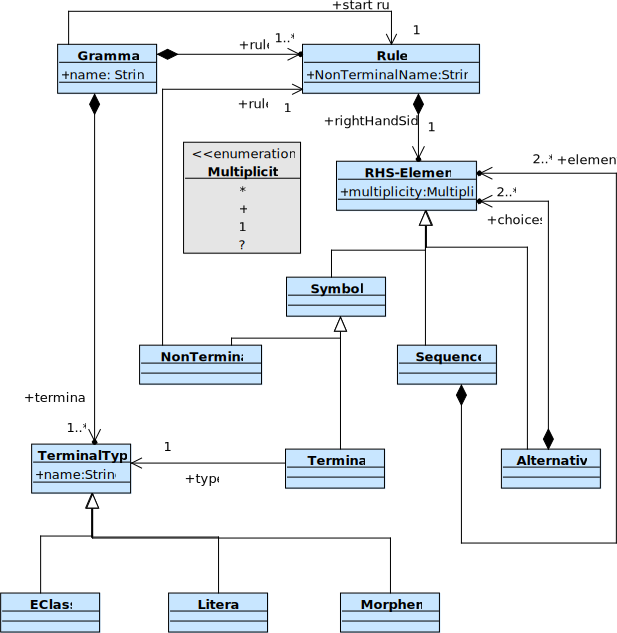
\includegraphics[scale=0.85]{gfx/ex/Grammar_CFG} 
\caption{EBNF Grammar Metamodel}
\label{MM:EBNF}
\end{figure}

Figure \ref{MM:EBNF} shows a metamodel for an EBNF grammar. The metamodel lacks the ability to define lexemes  \\
Compared to the definition of a CFG, the non terminals are the set of \code{NonTerminalName}s of \code{Rule}, the terminals are the set of \code{name}s of \code{TerminalType}, the start symbol is the \code{Rule} referred by \code{Grammar} and the productions are implicit described by the directly and indirectly contained elements of the \code{Rule}s. The \code{NonTerminal} and \code{Terminal} elements in the grammar are just references to the real non terminals and terminals. This definition overlap is owed to the fact that the same terminal may appear multiple times in productions, which must be distinguishable . This denomination allows for example in following rule
\\\begin{code}
A : b$_1$ C b$_2$
\end{code}\\
to be \code{b$_1$} an instance of \code{Terminal}, \code{C} and instance of \code{NonTerminal} and \code{b$_2$} another instance of \code{Terminal}, but refering to the same \code{TerminalType}.

The \code{Grammar} has at least one \code{Rule} and one \code{TerminalType}. The \code{Grammar} has exactly one \code{start rule}. The \code{Rule}s have a name and contain exactly one element as their \code{rightHandSide}. This element might be either a \code{NonTerminal}, a \code{Terminal}, a \code{Sequence} or an \code{Alternative}. \code{Sequence}s and \code{Alternative}s are containers for at least two \code{RHS-Element}s. \code{Sequence} are \code{a b c} or \code{(a b)+} for example. \code{Terminal} and \code{NonTerminal} hold references to their unique type they represent. \code{Symbol} just provides abstraction but does not add expressivity to the language itself. Every \code{RHS-Element} has a \code{Multiplicity}, so exactly one \code{1}, one or none \code{?}, zero or more \code{+} or any multiplicity \code{*} can be expressed. Subclasses of \code{TerminalType} are present to allow a more detailed specification of \code{TerminalType} in later models.


%%%%%% GrammarMM()	%%%%%%%%%%%%%%%%%%%%%%%%%%%%%%

%% Grammar Instance
\subsection{Grammar Example}
\begin{figure}
\centering
\includegraphics[scale=0.7]{gfx/ex/grammarExample} 
\caption{Example Rule ``A := (w |x y)+ B? | z C''}
\label{MM:GrammarExample}
\end{figure}
Figure \ref{MM:GrammarExample} shows the model instance of the EBNF metamodel \ref{MM:EBNF} of the grammar  \code{A := (w |x y)+ B? | z C}. The grammar rules \code{B} and \code{C} are left out, as well as the start rule reference. The references to the symbols \code{w}, \code{x}, \code{y} and \code{z} are replaced with the name of the referenced symbol.

\subsection{Attributed Grammar}
\begin{figure}
\centering
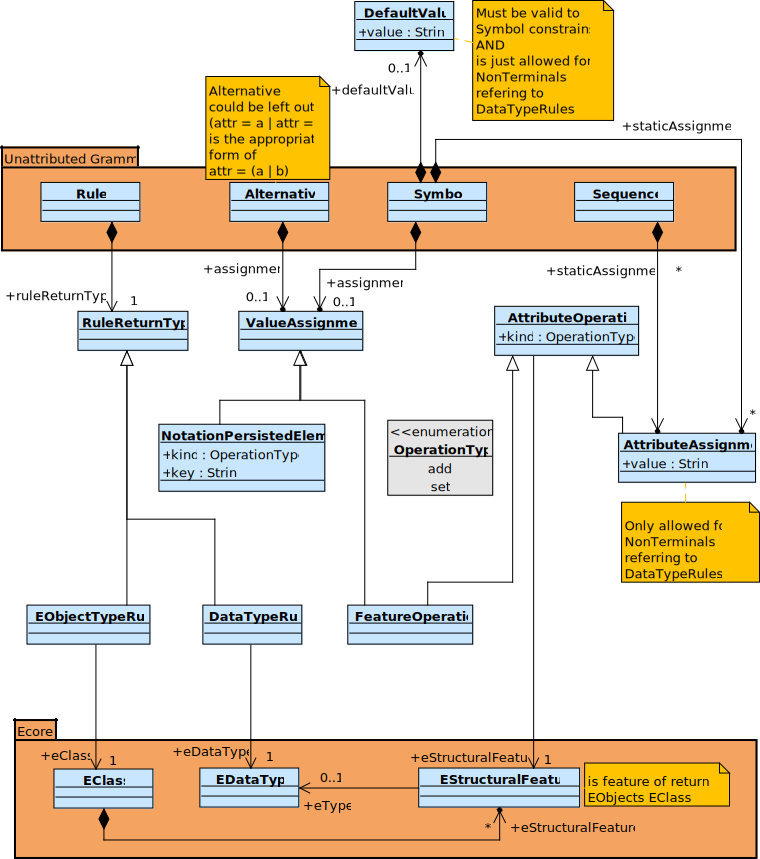
\includegraphics[scale=0.7]{gfx/ex/Grammar_Attributed} 
\caption{Attributed Grammar metamodel extension}
\label{MM:AEBNF}
\end{figure}

The metamodel defined in \ref{MM:AEBNF} adds attribution and default values to the grammar. It uses metaclasses from the metamodel \ref{MM:EBNF} for CFGs. The packaging is for documentation purpose only, because the metaclasses of the CFG metamodel refer to the current metaclasses. \\
Each \code{Rule} has a \code{RuleReturnType}, which might be an \code{EClass}, if it is a an \code{EObject} returning rule or an \code{EDataType}, if it is a Data Type Rule. The additionally distinction in \code{EObjectTypeRule} and \code{DataTypeRule} is for presentation purposes only, this makes it obvious in the diagram when an \code{EObjectTypeRule} is used. For a real implementation a reference from \code{Rule} to an \code{EClassifier} would be sufficient. \code{EClassifier} is the supertype of \code{EClass} and \code{EDataType}. \code{Symbol} now can contain a  \code{defaultValue}, which is a \code{String}.  \code{String}s are structureless, so the use of \code{DefaultValue}s is restricted to  \code{NonTerminal}s refering \code{DataTypeRule}s and  \code{Terminal}s only. The  \code{String} must not violate the  \code{Symbol}s constraints. Given the example \code{attribute+=TerminalSymbol}, an attribute assignment is realized by \code{TerminalSymbol} containing a  \code{FeatureOperation} with \code{kind} set to  \code{add} and a reference to the  \code{EStructuralFeature} named \code{attribute}. The \code{EStructuralFeature} must be contained in the  \code{EClass} of the returned \code{EObject}s type. In contrast to Xtext, it is possible to assign statically a structureless value to an attribute, for example 
\begin{xtxt}
Rule : {ruleAttribute="true"} "1"
\end{xtxt}   
which means that if the rule matches \code{ruleAttribute} is assigned to \code{"true"}. This can be done for an abitrary amount of \code{EStructuralFeatures}. \code{NotationPersistedElement} allows to persist a String in the notation model, this allows to share data between \code{Alternatives}. \\
\code{Alternatives} also contain a \code{ValueAssignment}. This could be omitted if 
\begin{xtxt}
attribute= (a | B)
\end{xtxt}
would not be allowed and instead only the alternative 
\begin{xtxt}
(attribute = a | attribute = B)
\end{xtxt}
would be allowed.
%% Grammar Instance()